\documentclass[11pt, spanish]{article}
\usepackage[utf8]{inputenc}
\usepackage{listings} 
\usepackage{graphicx}
\usepackage{amsfonts}
\usepackage[dvipsnames]{xcolor}
\usepackage[T1]{fontenc}
\usepackage{bigfoot}
\usepackage{amsmath}
\usepackage[numbered,framed]{matlab-prettifier}
\usepackage{caption}
\usepackage[figurename=Figura, tablename=Tabla, font={small,tt}]{caption}
\usepackage{blkarray}
\usepackage{xcolor}
\usepackage{multicol}
\usepackage[]{algorithm2e}

\makeatletter
    \setlength\@fptop{0\p@}
\makeatother

\date{}

\usepackage{geometry}
 \geometry{
 a4paper,
 left=30mm,
 right=30mm,
 top=30mm,
 }

\lstset{
	style              = Matlab-editor,
  	basicstyle         = \mlttfamily,
  	escapechar         = ",
  	mlshowsectionrules = true,
	framesep=4.5mm,
	framexleftmargin=2.5mm,
	fillcolor=\color{White},
	rulecolor=\color{Black},
	numberstyle=\normalfont\tiny\color{Black}
}

\captionsetup[lstlisting]{font={small,tt}}
\renewcommand{\lstlistingname}{Script}
\newcommand\RED{\color{red}}
\newcommand\BLUE{\color{blue}}
\newcommand{\BigO}[1]{\ensuremath{\operatorname{O}\bigl(#1\bigr)}}
\newcommand{\norm}[1]{\left\lVert#1\right\rVert}

\begin{document}

\renewcommand\lstlistlistingname{Lista de Scripts}

\author{Sebastián Valencia Calderón \\ 201111578}
\title{Tarea 2: Factorización de Cholesky y raices de un polinomio}
\maketitle

%====================================================================
\section{Introducción}

Los sistemas de ecuaciones lineales, aparecen en una gran variedad de aplicaciones en ciencia e ingeniería. Su naturaleza algorítmica, da lugar al diseño de herramientas computacionales para hallar la solución de estos sistemas. Existen dos categorías de los métodos que solucionan estos sistemas de manera secuencial. Los métodos iterativos y los métodos directos. Métodos como el de Jacobi, o Gauss-Seidel, pertenecen a la primera categoría, mientras a la última, pertenecen métodos más naturales, como la eliminación Gaussiana. De los diferentes métodos, interesan la eficiencia, es decir, la velocidad de convergencia y la exactitud de la aproximación de esta respuesta.\\

Un sistema lineal, se puede describir a muy alto nivel como un conjunto de ecuaciones lineales en varias variables. La representación natural que resulta conveniente en los métodos iterativos no es como anteriormente matricial, sino la algebraica general. Es decir, un sistema de ecuaciones de la siguiente forma:

$$ a_{11} \times x_1 + a_{12} \times x_2 + \dots + a_{1n} \times x_m = b_1 $$
$$ a_{21} \times x_1 + a_{22} \times x_2 + \dots + a_{2n} \times x_2 = b_2 $$
$$ \vdots $$
$$ a_{m1} \times x_1 + a_{m2} \times x_2 + \dots + a_{mn} \times x_m = b_n $$ \


Dado un sistema lineal algebraico, se pretende estudiar un conjunto básico de los métodos iterativos, de manera más precisa, los dos enunciados anteriormente: los métodos de Jacobi y de Gauss-Seidel. Con el desarrollo de estos ejercicios, se pretende cumplir con los siguientes objetivos:

\begin{enumerate}
\item Comprender la necesidad de implementación de métodos iterativos en la solución de sistemas lineales.
\item Implementar e identificar las características de diferentes métodos iterativos de solución de sistemas lineales.
\item Introducir casos de uso de sistemas lineales que requieren el uso de métodos iterativos.
\end{enumerate}

%==================================================================
\section{Procedimiento}

Para cumplir los objetivos enumerados anteriormente, se desarrollan algoritmos para resolver de manera iterativa sistemas de ecuaciones lineales, de manera específica, se desarrolla una función que implementa la iteración de Jacobi, y otra par implementar la iteración de Gauss-Seidel. Una vez los algoritmos están desarrollados y comprendidos, se procede a probarlos haciendo uso de un sistema lineal cuya solución analítica y algebraica es bien conocida, de tal manera que se puede comparar el resultado numérico obtenido a través de los algoritmos, y el valor conocido para distintos tamaños de la matriz (la comparación, se hace con los métodos de solución nativos en \textsc{MATLAB}). \\

Una vez se tenga comprensión de estos conceptos y de la geometría de las soluciones propuestas, se aplican los algoritmos para resolver sistemas de ecuaciones lineales que surgen en la vida real, de manera más específica, en la solución de circuitos lineales, donde se sabe que se trabaja con sistemas de ecuaciones lineales de a veces muchas variables.

%==================================================================
\section{Resultados}

A continuación, se exponen los resultados, las metodologías propuestas para los análisis y las herramientas de ejecución para cada uno de los problemas propuestos.\\

\begin{enumerate}
\item Se implementan en \textsc{MATLAB}, los algoritmos, uno para la iteración de Jacobi, otro para la iteración de Gauss-Seidel. Para garantizar un entendimiento completo y detallado, se incluye a continuación,  la deducción de los algoritmos. 

\begin{itemize}
\item \textbf{Métodos iterativos.} La solución de sistemas lineales de naturaleza dispersa y de gran tamaño, se ha convertido en un eje central de investigación en computación científica, y computación de alto desempeño. El tamaño de los problemas solucionados con este tipo de técnicas, aumenta con el paso del tiempo. Dentro de la categoría de métodos iterativos para la solución de sistemas lineales, existen dos sub-categorías, los métodos iterativos estacionarios, técnica inventada por Gauss, y los métodos iterativos no estacionarios, una metodología más moderna, que escapa del alcance de este informe. Una definición más precisa y exhaustiva, está contenida en \cite{heath2005scientific}. \\

Los métodos iterativos para la solución de sistemas de ecuaciones lineales, comienzan con una estimación de la respuesta $\hat{x}^{(0)}$, y sucesivamente, se mejora con base en las aproximaciones anteriores, hasta alcanzar una solución en el radio de convergencia deseado. Teóricamente, un número infinito de iteraciones es requerido, sin embargo, en práctica, las iteraciones pueden terminar al alcanzar un residuo, u otra métrica de error tan pequeños como se desee. Los métodos iterativos son fáciles de proponer, de implementar y en ocasiones, dependiendo de la naturaleza del problema, pueden ser muy eficientes.

\newpage

La deducción de los sistemas de interés, se muestra a continuación haciendo uso de un sistema general de tamaño 3. Dado el sistema de ecuaciones lineales:

$$ a_{11} \times x_1 + a_{12} + \times x_2+ a_{13} \times x_3 = b_1 $$
$$ a_{21} \times x_1 + a_{22} + \times x_2+ a_{23} \times x_3 = b_2 $$
$$ a_{31} \times x_1 + a_{32} + \times x_2+ a_{33} \times x_3 = b_3 $$\

A partir de ellas, es posible despejar para cada ecuación, la incógnita relacionada a ella: $eq^{(i)} \Rightarrow x_i$:

$$ x1 = \frac{\left[ b_1 - a_{12} \times x_2 - a_{13} \times x_3\right]}{a_{11}} $$
$$ x2 = \frac{\left[ b_2 - a_{21} \times x_1 - a_{23} \times x_3\right]}{a_{22}} $$
$$ x3 = \frac{\left[ b_3 - a_{31} \times x_1 - a_{32} \times x_2\right]}{a_{33}} $$\

Dado un vector inicial $\hat{x}^{(0)}$, se puede calcular el vector $\hat{x}^{(k)}$, en el sistema descrito anteriormente con la siguiente regla de sustitución:

$$ x1^{(k)} = \frac{\left[ b_1 - a_{12} \times x_2^{(k-1)} - a_{13} \times x_3^{(k-1)}\right]}{a_{11}} $$
$$ x2^{(k)} = \frac{\left[ b_2 - a_{21} \times x_1^{(k-1)} - a_{23} \times x_3^{(k-1)}\right]}{a_{22}} $$
$$ x3^{(k)} = \frac{\left[ b_3 - a_{31} \times x_1^{(k-1)} - a_{32} \times x_2^{(k-1)}\right]}{a_{33}} $$\

De manera análoga, es posible proponer la siguiente regla de sustitución iterativa:

$$ x1^{(k)} = \frac{\left[ b_1 - a_{12} \times x_2^{(k-1)} - a_{13} \times x_3^{(k-1)}\right]}{a_{11}} $$
$$ x2^{(k)} = \frac{\left[ b_2 - a_{21} \times x_1^{(k)} - a_{23} \times x_3^{(k-1)}\right]}{a_{22}} $$
$$ x3^{(k)} = \frac{\left[ b_3 - a_{31} \times x_1^{(k)} - a_{32} \times x_2^{(k)}\right]}{a_{33}} $$\

La primera forma de sustitución iterativa, es la de \textbf{Jacobi}, la segunda la de \textbf{Gauss-Seidel}. La deducción descita anteriormente, es una variación de la referencia \cite{rosloniec2008fundamental}, y de la referencia \cite{yang2005applied} . Una generalización natural que surge a partir de las anteriores ilustraciones para el método de Jacobi y el de Gauss-Seidel, son respectivamente:\\

\begin{algorithm}[H]
 \KwData{$A \in \mathbb{R}^{n \times n}\ |\ a_{ii} \in \mathbb{R} - \{0\}$}
 \KwData{$\hat{b} \in \mathbb{R}^n$}
 \KwData{$\hat{x}^{(0)} \in \mathbb{R}^n$}\
 
 \For{$i \in [1,\ 2,\ \dots,\ n]$}{
 $x^{(k)}_{i} = \frac{b_{i} - \sum_{j = 1}^{i - 1}\left[ a_{ij} \times x_j^{(k - 1)}\right] - \sum_{j = i + 1}^{n}\left[ a_{ij} \times x_j^{(k - 1)}\right]}{a_{ii}}$
 }\
 \caption{Iteración de Jacobi}
\end{algorithm}\

\begin{algorithm}[H]
 \KwData{$A \in \mathbb{R}^{n \times n}\ |\ a_{ii} \in \mathbb{R} - \{0\}$}
 \KwData{$\hat{b} \in \mathbb{R}^n$}
 \KwData{$\hat{x}^{(0)} \in \mathbb{R}^n$}\
 
 \For{$i \in [1,\ 2,\ \dots,\ n]$}{
 $x^{(k)}_{i} = \frac{b_{i} - \sum_{j = 1}^{i - 1}\left[ a_{ij} \times x_j^{(k)}\right] - \sum_{j = i + 1}^{n}\left[ a_{ij} \times x_j^{(k - 1)}\right]}{a_{ii}}$
 }\
 \caption{Iteración de Gauss-Seidel}
\end{algorithm}\

La referencia \cite{cheney2012numerical}, contiene una sugerencia para la implementación real del algoritmo. Con base en esta sugerencia, se implementan en \textsc{MATLAB}, los métodos iterativos de Jacobi y de Gauss-Seidel. El script \ref{lst:jacobi}, es una implementación del primer método (Jacobi), el script \ref{lst:gaussseidel}, implementa la iteración de Gauss-Seidel.

\end{itemize}

\item Para validar los algoritmos implementados, se propone el uso de una matriz tridiagonal, la cual, por su naturaleza dispersa (en inglés sparse), se presta para ser parte de un sistema de ecuaciones lineales que pueda solucionarse por medio del uso de los algoritmos implementados. El uso de los algoritmos implementados, se documenta en el siguiente script.

\lstinputlisting[caption = {Uso de los scripts previamente implementados.}, label={lst:usage}]{data/scripts/usage.m}

En este caso, con $k = 22$, la iteración de Jacobi converge a la solución, mientras la iteración de Gauss-Seidel, lo hace en $k = 10$. En ambos casos, el resultado (\texttt{xjac}, \texttt{xgas}), es:

$$\left(\begin{array}{c} 2.0\\ 3.0\\ -1.0 \end{array}\right)$$  

Dado un $n \geq 3$. $A \in \mathbb{R}^{n \times n}$ es una matriz tridiagonal, si tiene que posee únicamente elementos no nulos en la diagonal principal y en las dos adyacentes a esta, de resto, todos los elementos son $0$.

$$a_{ij} = 0 \leftrightarrow |i - j| > 1\ i,\ j \in \{1,2,\dots,n\}$$

Este tipo de matrices, aparecen frecuentemente en la solución numérica de ecuaciones diferenciales, y poseen la particularidad de que su factorización $LU$, es computacionalmente barata. Un ejemplo de este tipo de matriz es:\\

$$\left(\begin{array}{cccccccc} 4.0 & -1.0 & 0 & 0 & 0 & 0 & 0 & 0\\ -1.0 & 4.0 & -1.0 & 0 & 0 & 0 & 0 & 0\\ 0 & -1.0 & 4.0 & -1.0 & 0 & 0 & 0 & 0\\ 0 & 0 & -1.0 & 4.0 & -1.0 & 0 & 0 & 0\\ 0 & 0 & 0 & -1.0 & 4.0 & -1.0 & 0 & 0\\ 0 & 0 & 0 & 0 & -1.0 & 4.0 & -1.0 & 0\\ 0 & 0 & 0 & 0 & 0 & -1.0 & 4.0 & -1.0\\ 0 & 0 & 0 & 0 & 0 & 0 & -1.0 & 4.0 \end{array}\right)
$$\\

Más información relacionada con la forma en la que algunos algoritmos aprovechan esta forma, se encuentra en la referencia \cite{suli2003introduction}. Para validar la implementación, de los algoritmos, se crea un script de generación de sistemas lineales donde la matriz de coeficientes es tridiagonal. El script que materializa dicha intensión es el script \ref{lst:gensystem}. Los métodos para comparar con los implementados aquí, son:

\begin{itemize}
\item \texttt{inv(A) * b'}, el objetivo de esta expresión, es hallar la inversa de una matriz $A$, y multiplicar $A^{-1}$ y el vector $b$, para obtener el valor del vector $x$. El único parámetro de \texttt{inv()}, es la matriz a invertir, este no se implementa, reduciendo el sistema aumentado $[\ A\ |\ b\ ]$, y aplicando eliminación de Gauss, pues \textsc{MATLAB}, documenta demoras en la aplicación de esta función para resolver un sistema, pues interviene ademas, la multiplicación de matrices (\BigO{n^3 }).

\item \texttt{linsolve()}, recibe como parámetros la matriz $A$, y el vector $b$. Su funcionamiento, fue explicado anteriormente.

\item \texttt{rref()}, recibe como parámetro el sistema aumentado $[\ A\ |\ b\ ]$, y aplicando eliminación de Gauss, determina la forma escalonada reducida para obtener las respuestas requeridas.

\item \texttt{mldivide()}, recibe como parámetro la matriz $A$, y el vector $b$. Aplicando optimización de mínimos cuadrados, este llega a la respuesta en el caso de que $A$ sea no singular.
\end{itemize}

\newpage

La comparación, se hace con el script \ref{lst:validation}. Los residuos en cada caso, se relacionan en la siguiente figura, la metodología para relacionar los residuos, y los métodos, se consultó en las referencias \cite{isaacson1994analysis} y \cite{zalizniak2008essentials}.


\begin{figure}[htbp]
\centering
	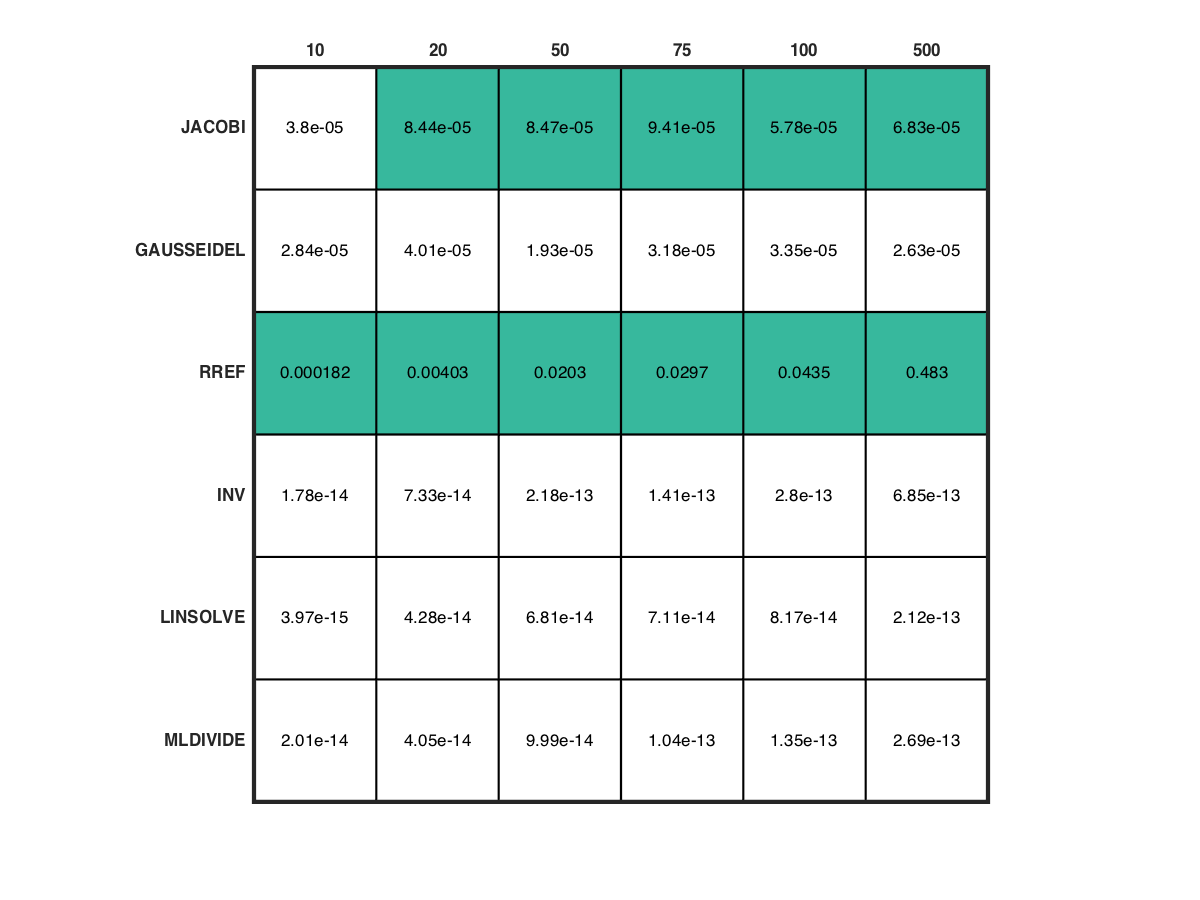
\includegraphics[scale=0.85]{data/img/comparisson}
	\caption{Errores obtenidos con la solución numérica y la algebraica de cada sistema para un orden o tamaño variante. El eje x es el tamaño del problema, y el eje y el error absoluto medido para cada método de solución.}
\end{figure}

Puede observarse que el peor desempeño según el error obtenido, es el de la forma escalonada reducid seguido por el método iterativo de Jacobi. Esto, puede deberse a la naturaleza del problema, pues una matriz de este tipo, es bastante fácil (rápido) de resolver mediante una factorización LU, la cuál se sabe, está respaldada por la eliminación de Gauss, que a su vez, respalda los metodos \texttt{inv}, \texttt{linsolve}, \texttt{mldivide}. Mientras que la eliminación de Gauss aprovecha la estructura o forma de la matriz, los métodos iterativos, no tienen en cuenta estos aspectos que pueden aprovecharse para mejor convergencia o reducir el error.

\end{enumerate}

\newpage

%==================================================================
\section{Conclusiones}

Mediante el desarrollo del laboratorio propuesto, se pudo verificar la importancia del diseño y análisis de algoritmos (en particular, los iterativos), en el álgebra lineal numérica o cálculo o álgebra matricial. Conocer algoritmos para resolver sistemas de ecuaciones lineales, permite hacer uso de máquinas digitales para implementar, obtener y verificar la solución de sistemas de ecuaciones lineales. Además de ver esto, se estudió otra metodología para la solución numérica de los sistemas de ecuaciones lineales, la metodología iterativa estacionaria, la cual tiene en cuenta las soluciones pasadas (Jacobi), o las presentes y pasadas (Gauss-Seidel), para llegar a una mejor aproximación de la solución. Conocer los métodos directos, y los iterativos para la solución de sistemas lineales, permite identificar la pertinencia de uso en los diferentes casos posibles. Ademas de esto, se puede concluir lo siguiente:

\begin{itemize}

\item La pertinencia de métodos iterativos, resulta precisa en matrices donde la estructura no en forma sino contenido, se pueda explotar, es decir, resulta más conveniente el uso de este tipo de algoritmos con matrices dispersas, lo cual puede llevar a una convergencia rápida en términos de eficiencia de recursos usados. Sin embargo, este tipo de matrices tiene una forma que puede ser explotada en cierta disposición (tridiagonal o en banda), a través de los métodos directos de solución. Conocer la forma y fondo de las matrices, resulta conveniente a la hora de determinar el mejor algoritmo a usar, o por qué es posible descartar algunos de ellos.
  
   \item El uso de aproximaciones iterativas a partir de un valor supuesto o adivinado, resulta una forma intuitiva de resolver un problema numérico, en este caso, la deducción es natural si se despeja la incógnita relacionada a cada ecuación. Esta sencilla observación, se presta para implementar un algoritmo robusto y estable que aprovecha el entendimiento del problema y las estructuras matemáticas detrás de el. Es decir, es demasiado importante para el diseño de algoritmos numéricos conocer la estructura formal o matemática de cada problema.
   
\end{itemize}


%==================================================================
\newpage
\section{Bibliografía}

\begingroup
\renewcommand{\section}[2]{}%
\begin{thebibliography}{}

\bibitem{isaacson1994analysis} Isaacson, E. and Keller, H.B. {\em Analysis of Numerical Methods.} 1994. Dover Publications - Dover Books on Mathematics. Página 61 - 62.

\bibitem{yang2005applied} Yang, W.Y. and Cao, W. and Chung, T.S. and Morris, J. {\em Applied Numerical Methods Using MATLAB.} 2006. Wiley. Página 98 - 103.

\bibitem{zalizniak2008essentials} Zalizniak, V. {\em Essentials of Scientific Computing: Numerical Methods for Science and Engineering.} 2008. Elsevier Science. Página 34 - 42.

\bibitem{suli2003introduction} Suli, E. and Mayers, D.F. {\em An Introduction to Numerical Analysis.} 2003. Cambridge University Press. Página 87 - 98.

\bibitem{heath2005scientific} Heath, M.T. {\em Scientific Computing: An Introductory Survey.} 2005. McGraw-Hill. Página 67.

\bibitem{cheney2012numerical} Cheney, E.W. and Kincaid, D.R. {\em Numerical Mathematics and Computing.} 2012. Cengage Learning. Página 322 - 328.

\bibitem{rosloniec2008fundamental} Rosloniec, S. {\em Fundamental Numerical Methods for Electrical Engineering.} 2008. Springer Berlin Heidelberg - Lecture Notes in Electrical Engineering. Página 17 - 27.



\end{thebibliography}
\endgroup

%==================================================================
\newpage
\section{Scripts}

\lstinputlisting[caption = {Iteración de Jacobi.}, label={lst:jacobi}]{data/scripts/jacobi.m}

\newpage

\lstinputlisting[caption = {Iteración de Gauss-Seidel.}, label={lst:gaussseidel}]{data/scripts/gaussseidel.m}

\lstinputlisting[caption = {Generación de un sistema lineal con una matriz tridiagonal.}, label={lst:gensystem}]{data/scripts/gensystem.m}

\newpage

\lstinputlisting[caption = {Solución de varios sistemas tridiagonales, haciendo uso de varios métodos.}, label={lst:validation}]{data/scripts/validation.m}

\addcontentsline{toc}{chapter}{\lstlistlistingname}
\lstlistoflistings

\bibliography{sample}

\end{document}
